\chapter{Methodology and Implementation}
\label{chap:metodology}

%goal 
To meet our goal for this project as outlined in~\cref{chap:introduction} we must create a method for identifying on-chain LN transactions within the blockchain, allowing us to discover what information is available in them. In \cref{sec:background} we covered how the LN uses the blockchain to operate with certain on-chain transactions. This means the on-chain LN transactions we will find are used to open, close, or claim founds related to a channel. As we are interested in what we can learn about the LN and its users from analyzing the blockchain, we will not utilize the information in non LN relevant transactions in this project. Reason for this is the size of the blockchain as discussed in \cref{sec:related}, which means the requirements for both software and hardware will be high if all information in the blockchian should be kept track of when parsing it. Potential benefits of using information from all transactions, LN related or not, will be discussed in \cref{sec:future} on future work. 
\\

%blockchain vs ln
With the LN being layered on top of Bitcoin, it requires the Bitcoin system to work, while the opposite is not the case. The LN will also be aware of the state of the Bitcoin system, as it uses the Blockchian to operate the channels. The Bitcoin system on the other hand is unaware of the LN and does not distinguish between on-chain LN transaction and other transactions. This means that when we use the Bitcoin Blockchian as the source of LN data, the amount of data will be smaller and not found in any LN context, compared to using the LN directly and collecting data from there. However, the LN is a dynamic changing network of nodes, channels, and payments; which is not stored in any public ledger like the blockchain. The information found in the LN can be recorded and stored by participants, but the system itself does not keep such a record. The data in the blockchain can be verified by any user as explained in \cref{subsec:blockchain}, while data recorded from the LN could not be verified in the same manner on its own.
This means that if we want verifiable historical data about the LN or to verify data collected from the LN, we must look to the blockchain. It will have limited and less information than what can be found in the LN, but will have the properties of being verified and automatically recorded by the Bitcoin system.
While the Blockchain is the approach used in the project, there will be benefits from using the fact that there is more information available by connecting to the LN and record data. Collecting data from the LN will allow us compare it with what we find on the blockchain. By doing this comparison we can verify and quantify the effectiveness of our method for identifying LN relevant transactions on the blockchain. Comparing the blockchain and LN data can also show what information we are unable to get trough the blockchain, or to what extent something is available in the blockchain.  
\\


\section{Blockchain analysis}
\label{blockchain_analysis}
%subgraphs representing channels
The transactions in the blockchain is linked with outputs - inputs forming a DAG as we explained in \cref{subsec:transactions}. Parsing the blockchain involves linking these transactions to form this transaction graph, allowing each transaction to be seen in context with every other. When applying the heuristics used by previous works discussed in \cref{sec:background}, one can use the results of this to provide additional context to the graph-i.e., when users are defined by key sets, the pseudonymous properties of using new keys for each transaction is removed, and so user activity is revealed. Because we are interested in transactions related to the LN, we do not create a complete transaction graph containing all transactions on the blockchain; instead we only link transactions related to a single LN channel, which creates many small transactions graphs, each representing LN a channel, and each a sub graph of the complete transaction graph. 
We will refer to these graphs as channel graphs because they contain the most common on-chain transactions related to a LN channel.
By only creating channel graphs and not the complete transaction graph, we do not need keep track as much data during parsing of the blockchain, which makes our task of analyzing the blockchain easier. 
In our project we use two methods for locating possible channel graphs: using timelocked redeem script, and using 2of2 multisig redeem scripts.
They are different, as the multisig method will get all potential channels, but will also give false positives, while the timelocked method is more reliable in terms of identification, but will not be able to identify as many channels.
Our focus has been on the timelocked method as because of the reliability, but multisig detection has also played a role.


\subsection{Using 2of2 Multisig for identification}
\label{detection_ms}

%identifying, craeting graphs
Channel graphs created using this method will contain the founding and closing transactions as shown in \cref{fig:ln_tx_graph_small}.
This will also be the case for all types of channel graphs, as it is these transactions that represents a channel on-chain.
To create the channel graphs when parsing the blockchain, we must be able to differentiate between on-chain LN transactions and other Bitcoin transactions. Therefore, we must find some characteristics needed or only found in on-chain LN transactions. 
In \cref{fig:ln_tx_graph} we can see some characteristics of the founding and closing transactions.
The output in the founding transaction used for the channel must be P2WSH, and the closing transaction will always have one input which will be a 2of2 multisig redeem script as explained in \cref{subsec:pcln}. The different characteristics have different levels of uniqueness, but using more unique characteristics will often impact the number of channels which can be identified, meaning there is a trade-off between specificity and broadness for identification. An example of this is the P2WSH output type, which is not very unique, so it will provide many false positives, but will allow for detection of both closed and open channels, which we will discuss more in \cref{subsec:information_ln}. 
The 2of2 redeem script is on the other hand more unique, as it is a specific redeem script and must therefore also belong to a P2WSH output - input pair. In the founding transaction we will only be able to check if it has any P2WSH outputs, while the closing transaction will allow us to check for the 2of2 multisig characteristic, which the presence of also entails the P2WSH characteristic.
Using closing transactions will limit us to closed channels, but the transactions matching our characteristics are more likely to be LN related. While the 2of2 multisig reedem script will be present in all closing transactions for LN channels, they can also be used for other purposes. We therefore cannot use this to determine with certainty if a transaction is a closing transaction or not, but it will rule out all transactions without this characteristic. So by locating all transactions having inputs with such redeem scripts, we will have all potential closing transactions, and by following the input - output connection we can also locate the founding transaction, providing us with a channel graph with the transactions as shown in \cref{fig:ln_tx_graph_small}.

\begin{figure}[h]
    \centering
    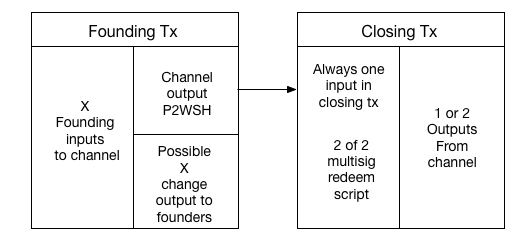
\includegraphics[width=10cm]{figures/ln_tx_graph_small.png}
    \caption{Channel graph with founding and closing transactions}
    \label{fig:ln_tx_graph_small}
\end{figure}

Creating channel graphs as explained above, identifies the transactions in the channel graph in reverse in relation to their creation order-i.e., we identify the closing transaction first, and use it to find the founding transaction. As stated before the transactions form a DAG, meaning they will be located chronologically in the blockchain, with newer transaction being found towards the tip of the chain. For the transactions in our channel graphs this means that the closing transactions will be found before the founding transaction, as the closing uses the output of the founding.
We must therefore parse the blockchain in reverse, beginning with the most recent block, and working towards the genesis (first) block.
This will ensure that we encounter the transactions in the order we want-i.e., closing transaction before the founding.
As explained in \cref{subsec:blockchain} the  blocks in the blockchain contains the hash of the previous block, which creates the chain connecting them. This provides a way of easily parsing the blocks and therefore also the transactions in the desired order. 
\\

The software we have developed for this project parses the blockchain and identifies relevant transactions, using both the multisig and timelocked identification methods.
We use the btcd \cite{btcd_roasbeef} Bitcoin implementation written in Go, for fetching and storing the blockchain data, and we also use its libraries to read the blockchain data in our software.
At a high level our software finds the latest block from the blockchain stored on disk and uses it as a starting point;
it then iterates over the transactions in the block, and checks if they are relevant for our project-i.e., is part of a channel graph. If that is the case they are stored in a channel graph structure. After all transactions in a block is parsed, the hash of the preceding block is used to fetch it from the disk, and the same process is repeated.
For each transaction it parses, it checks if the inputs have a 2of2 redeem script, if that is the case a channel graph is created and the transaction is stored as a closing transaction.
As explained in \cref{subsec:segwit} each transaction has a id, which is the transaction hash.
Transaction inputs references the hash of the transaction containing the output they spend, so when finding a potential closing transaction we get the hash of the corresponding founding transaction.
This is stored in a list, which we can use to recognize founding transactions when we encounter them in the blockchain.
This means we always check the hash of each transaction we parse, to see if it is is the founding transaction for a closing transaction we have already found. If there is a match, we have found all transactions for a single channel graph. This is the main algorithm for the software as can be seen in \cref{fig:algo1}, where the process described above is illustrated.

\begin{figure}[h]
    \centering
    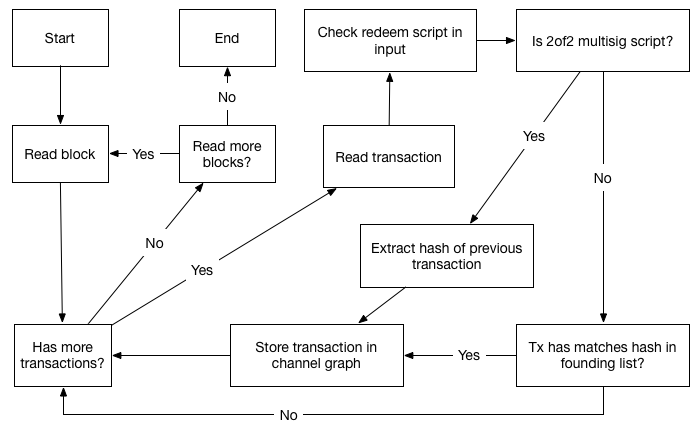
\includegraphics[width=12cm]{figures/algo1.png}
    \caption{Algorithm for parsing blockchain and creating channel graphs using the multisig method}
    \label{fig:algo1}
\end{figure}

The 2of2 multisig redeem script used to identify possible closing channels is shown below. Also a example of the byte version of such a script included, as this is how we get the script when extracting it from the input of a transaction, and therefore use when identifying the script.

\begin{verbatim}
2 <public key 1> <public key 2> 2 OP_CHECKMULTISIG
\end{verbatim}

\noindent [82 33 2 211 153 245 240 225 125 95 140 116 20 99 81 38 139 135 136 59 14 125 34 181 148 47 67 16 42 24 147 28 144 61 33 33 2 215 1 70 141 233 112 91 253 252 202 27 73 158 254 234 159 125 98 30 78 159 235 6 46 167 103 105 239 180 125 168 66 82 174]
\\

As we explained in \cref{subsec:scripts} the operations in Bitcoin scripts is called opcodes, and the Bitcoin wiki contains a list of all of them, and their encodings \cite{bitcoin_wiki_scripts}. The opcodes and their ordering in the script dictates the functionality of the script, so to identify a type of script we should look for scripts having the same format and operations.
We covered in \cref{subsec:scripts} and \cref{subsec:pcln} the purpose of this script is to create a scenario where multiple keys is required to unlock a output and spend it.
The scripts consists of of two numbers denoting the required and total number of keys required to create signatures, the public keys for the key pairs that can be used, and the checkmultisig operation. The required and total number of keys required will in our case be 2, as we are only looking for 2of2 scripts.
As shown above, the script starts with the required number of keys which must be used for signing, in this case 2, being 82 in the byte version. Then there is the first public key of the key pair able to sign. 
In the byte version the second vector is 33, which indicates how many bytes to push to the stack; this is the length of a compressed public key with prefix. Bitcoin uses elliptic curve cryptography, where a public key is two coordinates representing a point on the curve. The prefix for compressed keys can be 02 or 03, indicating if the y coordinate is even or odd \cite{antonopoulos2017mastering}. So the first byte vector in a compressed public key, and the third byte vector in this type of script will always be 2 or 3, and the 32 next bytes will be the rest of the compressed key <public key 1>. Then we have the other public key <public key 2> in the same format, followed by 2 or 82 in byte format, telling us the total number of keys which can be used for signing. At the end we have the opcode 174 OP\_CHECKMULTISIG, which checks signatures against the public keys. To identify this type of script we check if the opcodes are present at their expected locations in the script, and the total length of the script. This means we check if certain indexes in the byte array contains the data we expect-e.g., we would expect the last index in the byte array to contain 174.
\\

When using 2of2 multisig redeem scripts, which also entails using P2WSH for identifying potential channels, our result will contain all actual LN channels, but likely also many that are not. The effectiveness of this will depend on the current use-cases for 2of2 multisig transactions besides on-chain LN transactions, and how common these are. To determine the current effectiveness of this method, we will compare data from the blockchain with data gathered through the LN, and with results from our other method. This will allow us to quantify the actual number of channels identified using this method, compared to the amount of false positives.
The \cref{sec:ln_analysis} will contain a more in-depth discussion of this.

\subsection{Identification using timelocked outputs}
\label{timelocked_identification}

The main method for idenifying channels we have used in this project, relies on timelocked redeem scripts.
While being more unique than the 2of2 multisig redeem script, it will only exists on channels that is unilatrially closed-i.e., the channel was closed by one of the parties, and not cooperatively.
In \cref{fig:ln_tx_graph} we can see how a channel graph is structured when this method is used.
We still have the founding and closing transactions, but the closing transaction is also a commitment transaction, as it was used to close the channel.
When a commitment transaction is published the output to the entity closing the channel will be timelocked, as we explained in \cref{subsec:pcln}.
This was to enable the other party to spend the output using the revocation key, in the case of the commitment being revoked-i.e., any commitment other the most recent.
In the blockchain this is implemented using a P2WSH output, which have a redeem script containing a timelock, and a clause for the revocation key.
As redeem scripts is only avaialble in the input of the transaction spending the P2WSH output, similarly as with the 2of2 multsig redeem script,
we will find this script in the transaction spending the timelocked output. 
We will refer to this transaction as the timelocked transaction, which can be seen on the right in \cref{fig:ln_tx_graph}.

\begin{figure}[h]
    \centering
    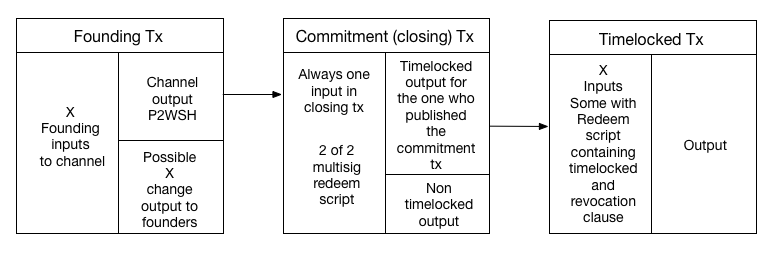
\includegraphics[width=15cm]{figures/chan_graph.png}
    \caption{Channel graph of unilaterally closed channel}
    \label{fig:ln_tx_graph}
\end{figure}

While the timelocked transaction containing the redeem script will not be present in channels closed cooperatively, 
the uniqueness of the the script will ensure the transactions that is identified using this characteristic are very likely to be actual timelocked transactions from the LN.
When a timelocked transaction is identified, we can use its input where we found the redeem script to get the hash of the closing/commitment transaction.
We can again use the input of the closing/commitment transaction to get the founding transaction. 
This way we be able to get all transactions in the channel graph.
We can also use the fact that the closing/commitment transaction will have the 2of2 multisig redeem script.
By checking that the closing/commitment transactions has this script in its input, same as we did in the multisig method, we are further ensuring we have found a LN channel.
Even with the timelocked scripts being very unique, because its specific use case, users are free to create the scripts they wish, so the presence of such a script will not guarantee that we have found a LN timelocked transaction.
While also LN related, we will see in \cref{subsec:htlc_onchain} how scripts having the same purpose being used in different transactions.
But by also checking that the closing transaction has the characteristics we expect, we can avoid instances where a timelocked script used in other scenarios.
\\

The identification and subsequent creation of channel graphs using this method, is implemented in our software in the much the same way as we described for the multisig method in \cref{detection_ms}.
To reiterate, timelocked transactions is identified using redeem scripts in their inputs, then the transaction hashes of the inputs is used to find the closing/commitment transaction.
The input of the closing transction is checked for the precence of 2of2 multisig redeem scripts, and if present the transaction hash of the founding transaction is used to locate it.
Each channel graph is created incrementally as we find each transacition it contains.
Instead of only having a list containing hashes of founding transactions, this method will also have a list of hashes for closing transactions.
For each transaction we parse, we first check if it is a timelocked transaction, if not, we check if its hash matches any found in the hash lists-i.e., check if it is a closing/commitment or founding transaction.
The lists are created as we locate timelocked and closing/commitment transactions and find hashes of previous transactions.
This whole process can be seen in \cref{fig:algo2}, which is similar to the one in \cref{fig:algo1} but more complex.

\begin{figure}[h]
    \centering
    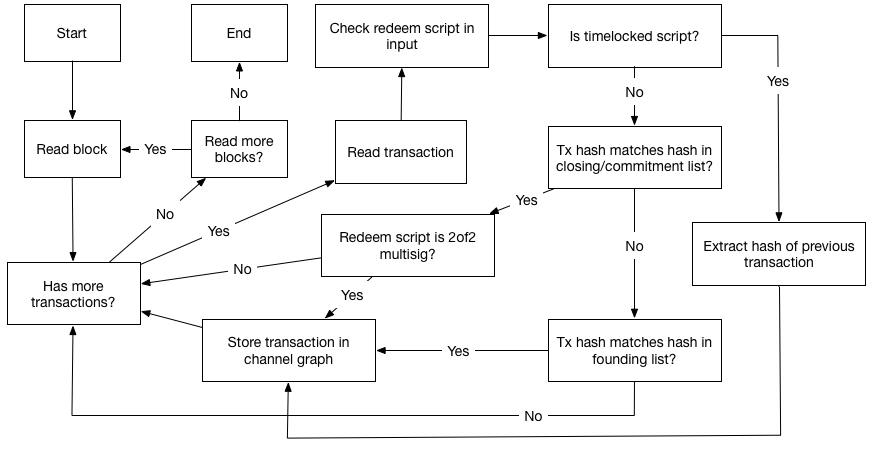
\includegraphics[width=12cm]{figures/algo2.png}
    \caption{Algorithm for parsing blockchain and creating channel graphs using the timelocked method}
    \label{fig:algo2}
\end{figure}

The timelocked redeem script \cite{bolt3} used to identify the timelocked transactions can be seen below:

\begin{verbatim}
OP_IF
    # Penalty transaction
    <revocationpubkey>
OP_ELSE
    `to_self_delay`
    OP_CSV
    OP_DROP
    <local_delayedpubkey>
OP_ENDIF
OP_CHECKSIG
\end{verbatim}

% timelocked script
The script contains a if - else clause, with the if clause being the one which allows the opposing party to spend the output in the case of the commitment transaction being revoked.  
In  \cref{subsec:pcln} we explained in detail how the parties will revoke old commitment transactions by exchanging keys, allowing the other party to spend the timelocked output with the key, and thus claim all the founds in the channel; this first clause is how this is done in practice.
A signature from the key pair of the <revocationpubkey> found in this clause, will make script evaluate to true, and thus allowing for the transaction to be spent.
The else clause is the timelocked portion of the script. It will contain the timelock, enforced by the CHECKSEQUENCEVERIFY operation defined in \cite{BIP112}, which will terminate the script if the specified delay has not passed. The delay is then removed from the stack with OP\_DROP such that a signature and public key are the only two items on the stack. Lastly OP\_CHECKSIG is used to verify the signature against the <local\_delayedpubkey>.
%The script will be located as the last item in the witness stack inside a transaction; see \cref{subsec:segwit} where we explained how the witness stack is structured for P2WSH transactions.
Below is the raw byte representation of a specific redeem script of the type shown above. Again, this is because our implementation handles the byte version of the scripts when identifying them. The byte version has been formatted in the same manner as the clear-text version, to allow for easier comparison.
\\

\noindent [99 \\
\indent 33 3 251 83 243 198 231 109 204 252 217 94 44 221 0 255 185 86 106 105 161 141 254 96 
\indent 167 77 48 16 57 146 128 4 80 1 \\
103 \\
\indent 82 \\
\indent 178 \\
\indent 117 \\
\indent 33 2 159 6 236 212 233 63 48 147 59 52 201 11 15 138 165 248 118 100 188 234 227 215 
\indent 108 160 135 22 57 37 117 250 172 130 \\
104 \\
172]
\\

%byte rep of script
The first byte vector seen in the byte script above is 99 which is the opcode for the the OP\_IF operation. The next vector is 33, which indicates how many bytes to push; As explained for the 2of2 multisig script: this is the length of a compressed public key with prefix. So the 33 next vectors will be the <revocationpubkey>. After this public key we will find the OP\_ELSE with the opcode 103, followed by the 82 'to\_self\_delay' which is the delay used for the OP\_CHECKSEQUENCEVERIFY (OP\_CSV) operation, having opcode 178. 
Next vector is 117 which is the OP\_DROP operation, and after we find the <local\_delayedpubkey> in the same format as <revocationpubkey>; 33 indicating the number of bytes to push to the stack followed by the prefix and the rest of the key. After that we have 104 which is the opcode for OP\_ENDIF, and 172 for OP\_CHECKSIG.
To identify this type of redeem script in timelocked transactions we check if the opcodes can be found at the expected locations. E.g., index 0 of the byte array should be 99 for the OP\_IF, and 103 for the OP\_ELSE operation should be at index 35, allowing space for a public key between it and the OP\_IF operation. Each opcode found in this script type is used for recognition, meaning all opcodes covered here must be present in the script for it to be identified as a timelocked redeem script, and they must also be found at their expected location relative to the others.
\\

As stated before, the inclusion of transactions in blocks naturally orders them, because transactions added in new blocks must have inputs from transactions already in the blockchain.
However, transactions pairs where one spends another can be confirmed at the same time, meaning they are included in the same block.
This occurs because the creator of the latest transaction spends a unconfirmed transaction-i.e., a transaction that has not yet been accepted as part of the shared transaction history of the network. 
Transactions are not necessarily ordered within blocks, so if two sequential transactions are located in the same block, we might encounter the latter transaction first.
This means we might encounter the founding transaction before the closing, but since we have not yet found the closing transaction, and therefore did not know the hash of the founding, we could not yet recognize it.
Because if this we had to iterate over the transactions in the block a second time if we found any transactions, to make sure we did not miss the preceding transaction earlier in the block.
Even with parsing some blocks twice the software parsed blocks fairly quick, parsing 100 000 000 transactions in under 90 minutes.
The memory consumption were also low, as our software only stored channel graphs and the hash lists for transactions we where currently looking for.

\subsection{HTLC on-chain}
\label{subsec:htlc_onchain}

In \cref{subsec:htlcln} we covered how transfers is facilitated within the LN using the HTLC construct. 
If the HTLC cannot be resolved off-chain, the channel will be closed and the HTLC will be handled on-chain.
This will a P2WSH output from the commitment/closing transaction, with a redeem script allowing users to spend it in two ways:
by either supplying the preimage R used to create the HTLC, or by waiting for the timelock to expire.


\todo{extra section. will remove if no time, but want some quick info about htlc's, need to reread about them. has results about them, so should be fairly quick to add to results, and a mention in results as potential method for more information. premiage R etc}

Our software is able to recognize these scripts, allowing us to check how commonly they occur, but does not actively use them as a identification method of channels.
The focus has been on using timelocked transactions, as the main method of identification, as it is a good combination of fairly unique and common transaction type in relation to LN channels. 
Our theory was that HTLC outputs, while being very unique, are rare compared to timelocked outputs, and that a large portion the channels they are found in also has a timelocked output.
But by being able to recognize them, we can see how rare they truly are, and as they are outputs of closing transactions we can see how many of them are outputs to channels we have found using the timelocked method.

%script + byte 

\subsection{Non implicit LN information on the blockchain}
\label{subsec:information_ln}
% how other information gathered. output types so on.

If we can successfully identify channel graphs containing transactions related to a LN channel, the data in those transactions will allow us to extract some information about the channel.
The value in the output - input pair used for the channel, will tell us the total value of the channel.
Timestamps is included in blocks when they are created, so by checking the timestamp of the blocks where the founding and closing transactions is located we can see how long the channel was active.
The number of inputs in the founding transaction and the number of outputs in the closing is also interesting; a founding transaction with a single input shows that a single user founded the channel; multiple inputs can indicate that both users founded the channel, but there is also a possibility that the channel is still founded by a single user, having multiple smaller outputs to get the desired value of the channel.
It is difficult to determine how founds have moved inside the channel based on value of the inputs to the founding transaction, and the value of the outputs from the closing transaction-i.e., it is hard to extract any information about any off-chain transactions by analyzing the outputs and inputs of the on-chain transactions.
The reason for this is that normally we can not determine which input/output belong to which user in the channel.
We discussed in \cref{subsec:scripts} how keys are used to lock outputs and signatures using those keys are used in inputs to unlock, meaning a key pair is related to a input-output.
In \cref{fig:keys_graphs} we have a founding transaction with two inputs (keys), a multisig output - inptut with two keys, and a closing transaction with two outputs (keys).
If we assume each user founded the channel with one input we can determine the initial balance between the parties by checking the value of those inputs.
Comparing that balance to the one in the two outputs will tell us how it has shifted from start of the channel to the end, but as discussed in \cref{sec:related} the pseudonymity provided by different key pairs makes us unable to see which of the inputs corresponds to which output.
We can also see in \cref{fig:keys_graphs} how the value is initially spread in two outputs then merged in the channel and then spread out again in two outputs, so simply following a specific value will not work.
Linking the keys used in these transactions as is done in previous work discussed in \cref{sec:related} will make this possible and is something we will discuss in \cref{sec:linking}.
The one thing we can determine by looking at inputs and outputs of a channel, without any key linking, is that a off-chain transaction has taken place in the channel, but this is only the case if there is one input to the funding transaction (single founded) and there is multiple outputs, meaning we know the channel started with with all value belonging to one party and it ends with the parties splitting the value.

\begin{figure}[h]
    \centering
    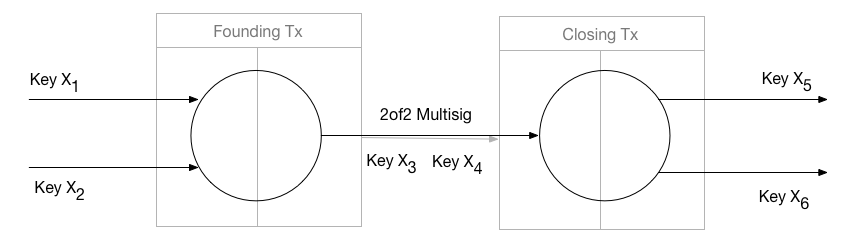
\includegraphics[width=14cm]{figures/keys_subgraph.png}
    \caption{Keys in a channel graph}
    \label{fig:keys_graphs}
\end{figure}

We discussed in \cref{detection_ms} how using P2WSH outputs would allow us to identify possible open channels, as all outputs used for LN channels are of this type. With the characteristic being fairly common we will most likely have many false positives, but we can use this fact to determine the maximum size (number of channels) of the LN.
By counting the number of unspent P2WSH outputs we will get maxium number of channels open. This can also be done to get the maximum number of LN channels at any historical point of the blockchain;
by counting all P2WSH outputs and subtracting the spent ones up to a height on the blockchain will get us the unspent outputs at that point.
While this might not be accurate in terms of actual number of channels (size) for the LN, it will give us a concrete upper limit to its size, both current and at any point in the past.
We can also use LN data to correlate between the number of unspent P2WSH outputs and open channels in the LN at different points in time. Which will indicate how closely the number P2WSH outputs reflects the number of LN channels.

\section{Lightning network analysis}
\label{sec:ln_analysis}

% lnd introduction
This project focuses on exploring the LN and related data trough the blockchain, but we can also use other approaches to verify and provide context to our view from the blockchain.
One such approach is simply to collect data from the LN directly.
This data will be more complete than what we can find on the blockchain, so it will provide us with the bigger picture. By comparing blockchain data with data directly from the LN, the effectiveness of our methods can be measured. In \cref{detection_ms} discussing our multisig detection method, we stated that it would create some channel graphs which where not actual LN channels. By comparing the potential channels we find using this method with the ones gathered directly from the LN we can determine the how many of our results are false positives.
The data from the LN can also provide us with the ideal result of linking information found on the blockchain. This is because some relations are explicitly defined in the LN data, but only implicitly or not at all on the blockchain, which makes our linking efforts on the blockchain data also measurable.
\\

To collect data from the LN we used the one of the implementations following the BOLT specification \cite{bolt}, called LND \cite{lnd}, which we modified to collect the data we where interested in. The LND implementation maintains a view of the current LN by storing a graph containing active channels and nodes. This is continuously updated as new channels are announced trough the network, and closing transactions is found on new blocks on the blockchain. It requires a Bitcoin instance running to interact with the Bitcoin network, which is used to publish on-chain transactions and monitor the blockchain. New channels are discovered by announcements within the LN, while channels closing is found by locating closing transactions in new blocks from the Bitcoin network-i.e., transactions spending outputs of founding transactions. 
Because the software already stores all channels and related data, we only needed to make it keep old data.
To do this we modified the 0.4.1-beta version of LND to create a copy of its database each time a new block notification was received from the Bitcoin software. This was not done immediately but within a minute so the changes from the block could be applied to the graph data. Doing this gave us a set of databases containing the state of the network at each block, essentially a set of snapshots of the LN.
\\


The snapshots contains the graph describing the state of the lightning network as known to our node at the time of the snapshot, so by comparing the graphs of different snapshots we can see how the network evolves over time. 
Each graph in the snapshots is essentially a set of channels active at that time. Consider two sets of channels representing the LN at different points in time: \(\kappa\) being the older and \(\tau\) the newer. The channels not present in \(\kappa\) but present in \(\tau\) would be new channels-i.e., the relative compliment of \(\kappa\) in \(\tau\), \( \tau \backslash{}\kappa\). Similarly the channels closed would be the ones present in \(\kappa\) but not in \(\tau\)-i.e., the relative compliemnt of \(\tau\) in \(\kappa\), \(\kappa\backslash{}\tau\). Doing this for each snapshot we can get a set of channels closed and opened during the data collection interval, and because we collect snapshot at each new block, we can easily contextualize the results with different blockheights-e.g., create a list of closed channels for each block, or number of active channels for each blockheight. This also makes it easy to compare data from the LN to data from the blockchian as we can use the blockheight as a index, ensuring we compare correct data.
Using some libraries from the LND implementation we created software to read the data generated by the node software, compare the snaptshots, and produce outputs with relevant information.
\\

% IF TIME CHANNEL ID used for comparsion 

One modification we made to the LND implementation besides generating snapshots for the network state, was removing the process of pruning the "zombie" channels from the graph. According to the BOLT rfc \cite{bolt7}, nodes can remove channels if the last channel update is older than two weeks. This is done to avoid open but abandoned or unusable channels to remain in the graph and be propagated to others. The LND implementation follows this recommendation and does this regularly. Our reasoning behind disabling this for our node was to keep data from the LN consistent with the blockchain data. Pruning channels would make changes to the LN graph, making it seem like channels where closed when they from the blockchain perspective where still open. Because we are focusing on the blockchain in our project, and are not interested in the routing availability of channels in the LN, we choose to keep these channels in the graph.

\section{Linking and key reuse}
\label{sec:linking}

% intro clusting, goals and related work
Linking or clustering information that is related has been the focus of much of the related work described in \cref{sec:related}. The main goal when doing this is to reveal non-explicit information, which in the context of the Bitcoin transaction graph would be constructing user profiles. 
This is done by linking keys controlled by the same user, which will counteract the pseudo-anonymous properties of the Bitcoin system. In our project we are only interested in the subset of Bitcoin users that is also LN users, in addition to information about the LN itself. 
Our methods for locating this relevant information have been outlined in \cref{blockchain_analysis}, the result of which is channel graphs containing the on-chain transactions related to one LN channel. 
As we do not take the entire Bitcoin transaction graph into consideration we are limited to using the data found inside channels graphs for linking. The main focus of linking in this project is to find relations between channel graphs, allowing us to link them based on shared user participation.
It relies on the fact that to be a usable network, the LN will need some nodes/users to have multiple channels to different users-i.e., some vertices will need to be of a degree higher than one. This relation between channels is clearly visible from the LN perspective, as the view of the network will contain this relation, but this is not the case for the blockchain. As we stated in the start of this chapter, the Bitcoin system is unaware of the existence and state of the LN, meaning the there is no explicit relation based on common nodes/users participation for channel graphs on the blockchain. As the on-chain LN transaction are mainly for managing channels, we are limited to linking information about channels or users within the channels. The off-chain transactions will by their very definition not be available to use for any linking.
\\

%defining a user
While we can link channels based on a common user participating on both, we can not determine which of the two users in either channel creates this relation. 
The reason for this is the same as discussed in \cref{subsec:information_ln}, where we pointed out the problems of matching inputs to outputs of a channel, to see changes in balance between the users. 
In previous works we discussed in \cref{sec:related} users where defined by control of a key pair, so essentially a key is a user.
Linking keys will reduce the number of users by redefining users as a set of key pairs.
E.g., a transaction graph with four keys, would mean there was four potential users, unless we managed to link keys which would reduce this.
For our case with the channel graphs, a problem arises because we know in advance how many users is involved in the graph.
There is two users involved in a channel, but usually many more keys present, so we have a reduced user count, but this is not due to linking keys. Defining a user in this setting is harder, as we cannot simply choose a arbitrary key for each of the two users. In \cref{fig:keys_graphs} we see how there are 6 keys which normally could each represent a user, but in our setting we know there is only two users. If we could link the keys, resulting in two sets of keys, then these sets could be our definition of a user as it would enable us to distinguish the users. But without two key sets, when linking channels based on a property in the channel graph, we cannot determine which of the users this property belongs to as we have no clear definition of the users.
We will however discuss later in this section some possibilities for defining users.
\\

We have used three heuristics for linking channel graphs in this project.
These are only for linking channel graphs based on common user participation; two of them can however be related to the heuristics discussed in \cref{sec:related} used in previous work. The heuristics employed are:

\begin{enumerate}

    \item \textbf{Key reuse}\\
This heuristic is simply to check if the same keys is present in different channel graphs.  
Any key found within a channel graph is sure to belong to one of the two users participating in the channel, so if the same key can be found in another graph we know the user owning the key participated in both channels.
This heuristic becomes useful because we are linking sets of transactions-i.e., transaction graphs representing channels. In previous work where they where linking keys, this becomes redundant as a key is obviously related to itself, but in our case we are not interested in keys as such but rather how they reveal user involvement. Because we know there is only two people participating in transactions within the channel graph, keys from any transaction inside the graph can be checked for reuse. The keys used in the founding and closing transactions clearly belongs to the participants, but with the timelocked transaction we cannot be so sure. The BOLT rfc \cite{bolt5} heavily recommends the owner to spend the timelocked output when it expires to transfer the value to a convenient address, reason being the redeem script required to spend the timelocked output, so the advanced script must be kept until the output is spent, which is inconvenient compared to having the value available in a normal P2WPKH output.
Assuming implementations follow this recommendation, the timelocked transaction and the keys found within should only contain keys related to the user which claimed the timelocked output. We should however note that the key reuse needs to happen in different channels, as key reuse within a single channel does not allow us to link any channels.
\\

    \item \textbf{Graph connections}\\
This heuristic is based on channel graphs being directly connected with each other with output - input pairs. Such a connection can be found in any outputs going to transactions outside the graph. 
This means all outputs in the founding transaction except the 2of2 multisig used for the channel, the non timelocked output in the closing transaction, and the outputs of the timelocked transaction can all be used for linking. 
In \cref{fig:linking_graphs} we can see these connections-e.g., the non-channel output of a founding transaction is used for input in another founding transaction. The reason we can determine shared user participation in connected channel graphs is that they are directly connected.
By inferring the purpose of outputs from the channel graph we can determine that the outputs are controlled by the participants in the channel, so if they connect to another graph we can say there is common user participation.
This concept is the same as the one used in previous work with heuristic 2 discussed in \cref{sec:related}, where some outputs from a transaction was assumed to be change for the sender. The non channel outputs of the founding transaction should be change back to the participants, as they may not want to use the entire value of the inputs in their channel. It is unlikely that the outputs is a transfer of funds to another entity unrelated to the channel, so we can safely assume that the outputs are controlled by one of the entities in the channel, so if they are used as input in another channel, it would tell us that the same user is participating in both. For the non timelocked output in the closing transaction, we know it must be controlled by one of the users as it is how the channel works. The control of the outputs of the timelocked transaction is based on the recommendation from the BOLT rfc \cite{bolt7} discussed in the previous heuristic. 

    \item \textbf{Graph overlap}\\
The third heuristic is when channel graphs overlap with each other, meaning a single transaction is part of multiple graphs. This can only occur with the timelocked transactions, as founding and closing transactions are used for controlling a single channel. This can change change however as we will discuss further in \cref{sec:future} on future work. We can see this overlap illustrated in \cref{fig:linking_graphs} where the timelocked transaction in the top right has inputs from two commitment/closing transactions and will thus be part of both channel graphs. This relates to heuristic one used in previous works as outlined in \cref{sec:related}, where transactions with multiple inputs was used to link keys used in those inputs. By being part of multiple graphs, a timelocked transaction will have multiple inputs. Which according to the old heuristic 2 tells us that the same user in control.
    
    
\end{enumerate}

\begin{figure}[h]
    \centering
    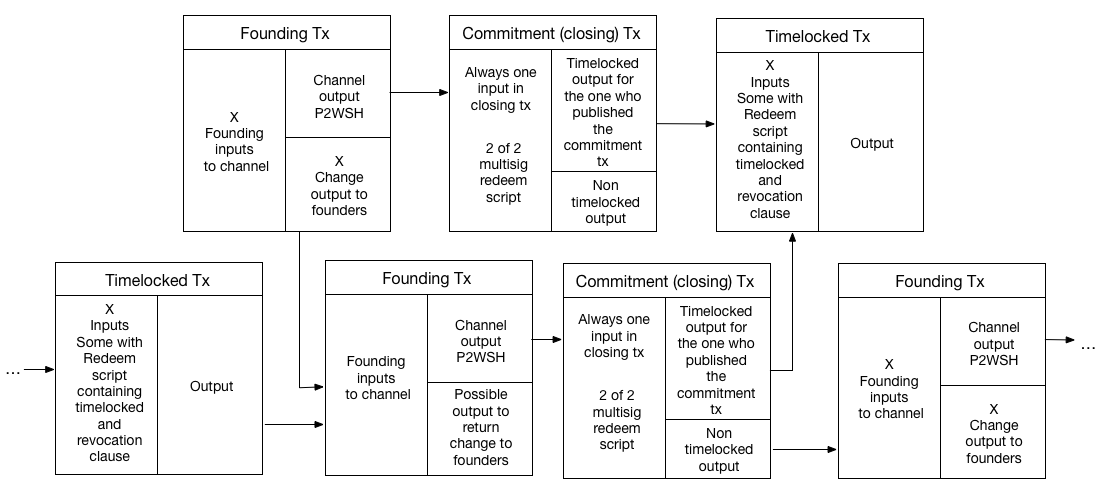
\includegraphics[width=14cm]{figures/graph_linking.png}
    \caption{Connected channel graphs}
    \label{fig:linking_graphs}
\end{figure}

%channel linking creating a channel graph
Linking channels based on shared user participation allows us to create a channel network visualizing how the channels are related to each other.
In this graph the vertices represents channels and the edges represent users/nodes in the LN.
While the transaction graph for Bitcoin allows us to see how founds are moving by giving us the structure of the transaction graph, 
the channel network can show us how founds can flow between channels based on their connection by users.
As the LN is a network itself, it has a natural graph structure where vertices are users/nodes and the channels is edges between the users, which we will refer to as the LN graph.
This is the reverse in terms of vertex - edges compared to our channel network. Another difference between the LN graph and our channel network graph, is that the LN graph requires distinction between users/nodes as the vertices in that graph is a specific user; in our channel network the edges is any of the two users participating in the vertices connected to the edge.
\\

%key reuse in same graph
%using ms keys to define users
Having a clear definition of users in the context of channels identified on the blockchain, will as discussed allow us to differentiate the users, meaning we can determine which channels a specific user participates in. This would allow us to crate a network using channels we have identified on-chain, having the same structure as the standard LN view-i.e., vertices representing users and edges being channels. Including the temporal aspects of the channels would allow one to recreate the structure of the LN at different points in time. 
One approach to achieving a clear distinction between the two users in the channel graphs is to disregard keys and related transactions; if we only use the 2of2 multisig output-input constituting the channel, we will only have two keys, one for each user. While this removal of information gives us a clear definition of a user in the channel, it also removes many possibilities for linking the channel to other channels. The only heuristic still viable if we only consider the channel output-input is key reuse of the keys used to define the users. This means we will not be able to link as many channels as previously, where we would have more keys to check for reuse, in addition to two other heuristics. Another possibility is to link all keys within a channel graph, resulting in two sets which each can represent the user as we discussed previously. This approach would allow us to use the heuristics presented above and also differentiate user participation. A hybrid between the two would also be possible: linking keys to the extent we are able to, and then disregarding information related to the keys we are unable to link to any set. The heuristics could still work using this approach, depending on the extent we are able to link keys, and which keys we are able to link. Linking keys should be done by using the entire transaction graph, as doing this will provide more linking possibilities than only taking the few transactions inside the channel graphs into consideration. This will be discussed more in \cref{sec:future} on future work.

%key reuse and, graph overlap
%The heuristics discussed in \cref{sec:related} used for previous works, where created for linking key pairs, found inside a output - input which again is located in a transaction. This meant the transaction was the largest unit taken into consideration when using the heuristics-e.g., a transaction has two inputs, indicating the keys used in both output - input pairs belong to the same user. In our case we have units consisting of multiple transactions which is the subgraphs representing a channel on-chain, but some of the general idea behind the heuristics is still relevant for our use. 
%
%If we take heuristic 1 from \cref{sec:related} as a example: it was based on transactions with multiple inputs, and how they could be used to determine that the keys used for these inputs belonged to the same user.
%With key pairs being used in a output - input as discussed in \cref{subsec:scripts}, we can also determine using this heuristic that the same user participated in multiple output - input pairs. In our case this can be used to finding a such pairs in different subgraphs, thus finding a common user participating in different subgraphs. This means we will check for transactions within the subgraphs having multiple inputs from different subgraphs, which will allow us to link the channels. 
%
%
%We have used three total heuristics for linking channels in our work, two of them are based on the previous ones described in \cref{sec:related}, while the third is more specific for our case.
%These three heurisitcs can bee seen in \cref{fig:linking_subgraphs} and is described below:
%
%\begin{enumerate}
%
%    \item \textbf{Outputs from multiple subgrahps being inputs in one transaction} (green circle) \\
% The first heuristic is having multiple inputs from different subgraphs in the same transaction, same as we discussed in the paragraph above.
% It is in the timelocked transaction this 
%    
%    \item \textbf{Change output used as input in another subgraph} (blue circle) \\
% The second heuristic is based on heuristic 2 discussed in \cref{sec:related} where some outputs was considered to be shadow addresses used by the creator of the transaction to receive change. Because we know there are two users participating in a subgraph and the purpose of the transactions is to operate channels, the outputs from the founding transaction going "outside" the subgraph should be to receive change from the creation of the channel. If this change output is used as input for a transaction in another subgraph we can link the two based on this.
% The only transactions in the subgraph which uses inputs from "outside" the subgraph is the founding input transactions, so it is here we will potentially find the output - input connection from the founding transaction in another subgraph.
% Theis heuristic is one of the main reasons we include the founding input transaction transaction in the channel subgraph. As these transactions provide the input to the founding transaction, at least the outputs used for this are controlled by the participants in the channel, and therefore if they use a output from another channel we can determine the same user was present in both. 
% 
%    \item \textbf{Key Reuse in different subgraphs} (red cirlce)\\
%    
%    
% \item \textbf{Same transactions present in multiple graphs} (ssss) \\
% As mentioned in \cref{sec:bc_analysis} the timelocked transaction in one subgraph can even be the founding input transaction in another, meaning the founding input can also provide overlap with the transaction graphs and not just a direct link with input - outputs.
% 
%\end{enumerate}
%%todo, single founded tx, linking not possible if all founds tranasferred.
%Defining a user when linking channels and using all information in the subgraph was problematic, but we can avoid this by only considering the keys in the 2of2 multisig output - input pair at the core of the channel subgraph. Using only these two keys will allow us  to differentiate the two users, and if any of the two keys is reused in other 2of2 multisig channel output - input pair we can determine which of the users is present in the other channel. Having clearly defined users we can identify in different channels would allow us to create a network where users is linked by participation in channels, similarly to the channel graph but here we can differentiate the users.
%In such a network nodes would be users and edges channels between them, giving us the a network with a view like the standard LN view. However, when only considering this single output - input pair we have very little information to use for linking; we can not use the rest of the transactions in the subgraph as we run into the differentiating users problem again if we are unable to link the keys in the subgraph, so in our tests we have only done linking based on key reuse in the 2of2 multisig channel input - output. 
